%% EXERCICIOS PARA INCLUÍR DENTRO DO CADERNO DE EXERCICIOS %%
%
% EXERCICIO.- ANÁLISE DA SECUENCIA: Dies irae
%
\section{Análise da secuencia <<Dies irae>>} \label{Intro}
%
Unha das secuencias máis coñecidas é o <<Dies irae>>, que no século XV empezouse a considerar parte da misa de defuntos, converténdose cara finais de século, nun movemento obrigado desta misa.

Para realizar a análise con partitura da audición desta secuencia, seguiremos os pasos indicados na analise de audición do <<Puer natus est>>  (ver o punto \ref{sec:Puer-natus} da páxina \pageref{sec:Puer-natus}); unha vez realizada a análise da partitura e escoita activa, completaremos os datos da obra.
\par
\vspace*{0.15cm}
%
% ----------------------
% Partitura de audición:
% ----------------------
\begin{figure}[h]
    \centering
    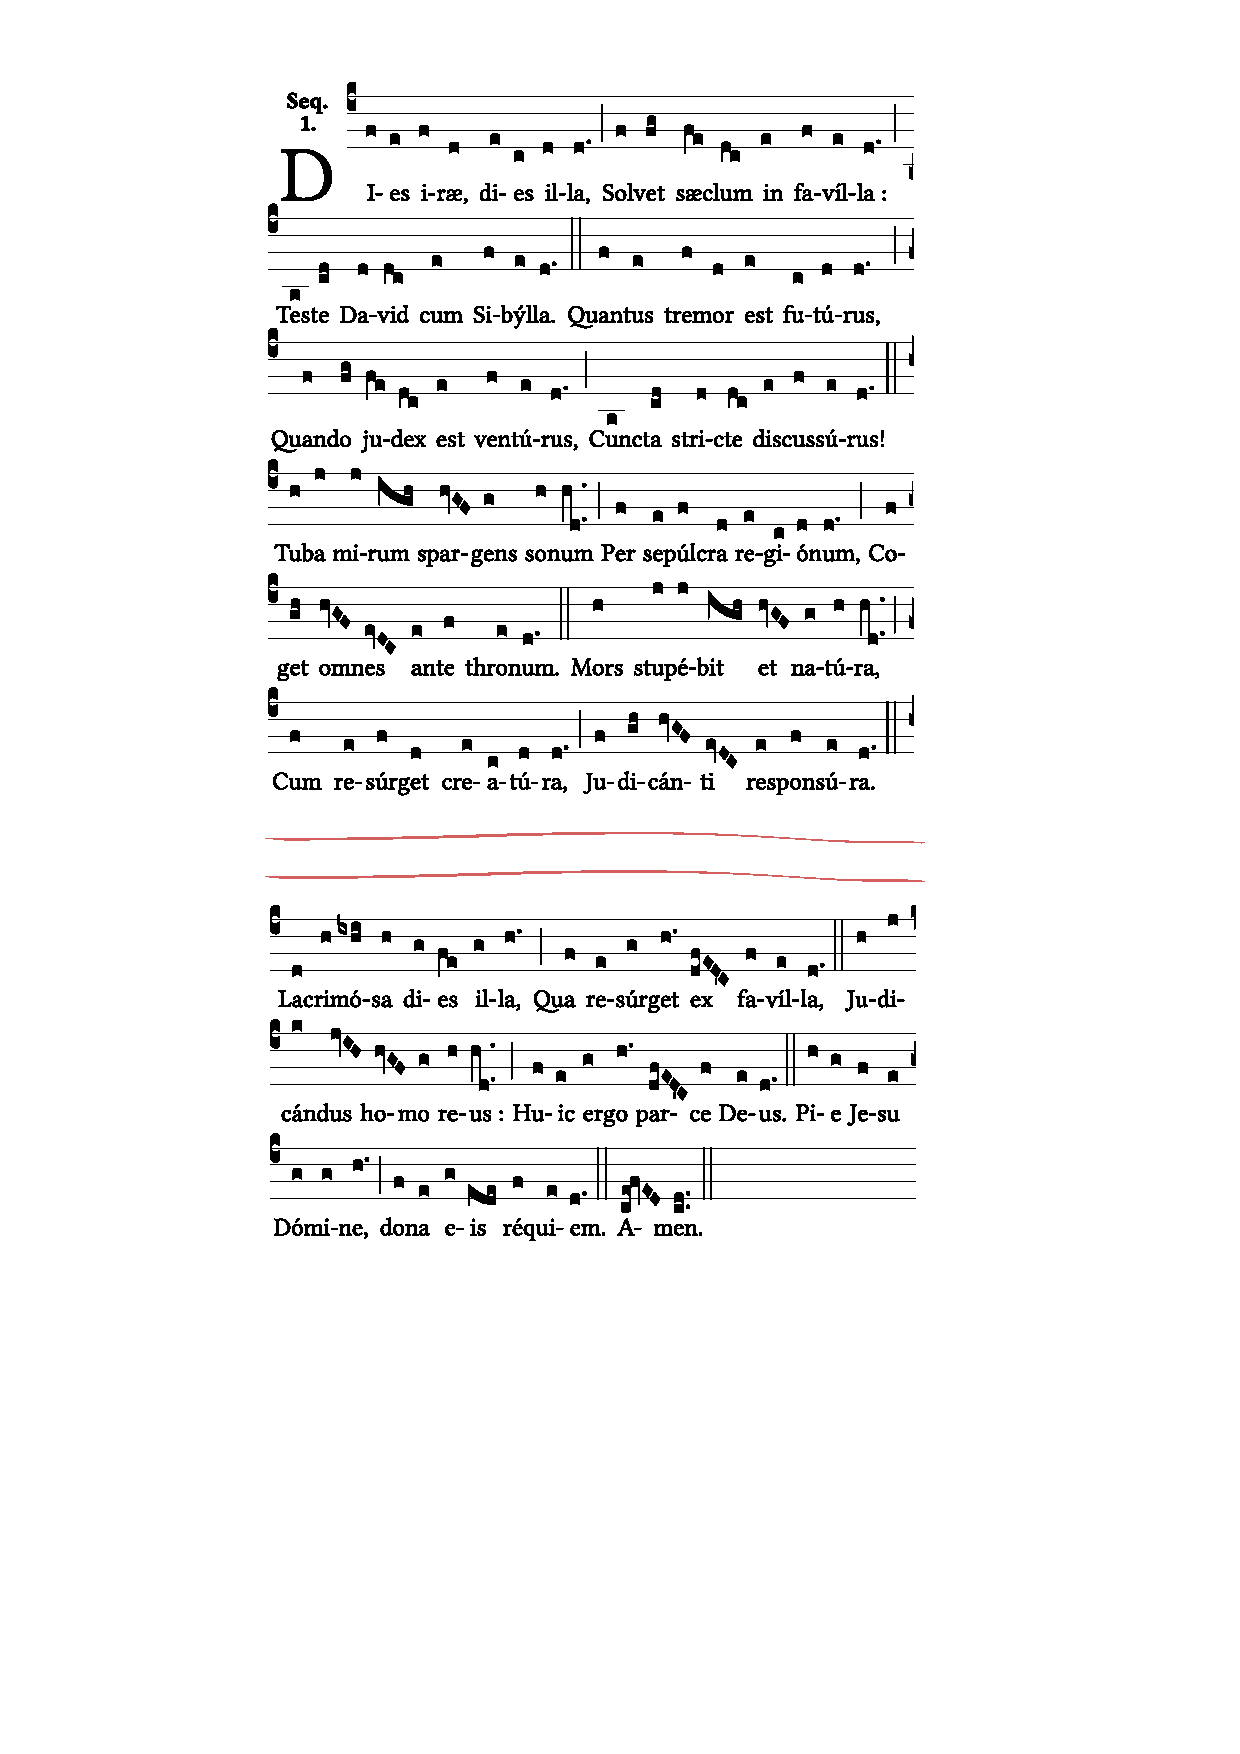
\includegraphics[width=0.60\textwidth]{figures/ud-03/dies-irae-solesmes-cut.pdf}
    \caption{Secc. do inicio e fin do <<Dies irae>>}
    \label{fig:dies-irae}
\end{figure}
% -----------------------
%
%\par
%\vspace*{0.25cm}
% INTRODUCCIÓN
% TODO: Revisar !!
%
%Trátase dunha peza monódica con texto en latín, sen ritmo estruturado, de estilo silábico, con unha estrutura de repetición que se podería representar co seguinte esquema: a bb cc dd e. 
%A primeira frase cántase unha soa vez, pero a segunda, terceira e cuarta cántanse dúas veces con textos diferentes. A música é diferente para cada frase. Termina cunha pequena frase que se canta unha soa vez.

%Polo xeral estas pezas distínguense por ser silábicas e, sobre todo, ter frases de música que se repiten por pares. A maioría teñen unha soa frase ao principio e ao final, e pares de frases intermedias. 
%En qué consiste a repetición pareada?
%As frases en pares repiten a melodía, pero o texto cambia. A forma é a bb cc dd ee… nn. Moitas secuencias son pezas moi longas, por exemplo o dies irae, mentres que unhas poucas, como o victimae paschali laudes, son curtas.
%
%\subsection*{Análise da audición} 

\begin{multicols}{2}

%\begin{enumerate}[1.-]
%PUNTO NÚMERO 1: ESCOITAR A PEZA
%
%\subsubsection*{Paso no. 1: análise da partitura} \label{analise-partitura}
%
%No caso de análise dunha audición con partitura prestaremos atención a tódolos elementos formais que observamos na partitura (notación e demáis grafías); son os primeiros elementos a recoñecer a golpe de vista.
%Aqueles elementos que son descoñecidos ou non recoñecemos a simple vista, rodearémolos cun círculo para aclarar o seu significado.
%
%\subsubsection*{Paso no. 2: escoita activa} \label{escoita}
%
%Despois da observación e lectura e identificaremos os elementos formais por medio dunha escoita activa da obra.
%É moi importante identificar auditivamente todo o que observamos no paso \ref{analise-partitura}.
%A escoita activa, axudaranos a determinar a relación música-texto da obra neste caso.
%
%\subsubsection*{Paso no.3: datos da audición} \label{datos-audicion}
%
%Unha vez realizados os pasos \ref{analise-partitura} e \ref{escoita} prestaremos atención aos seguintes puntos.
%
    \begin{enumerate}[1.-]
% ANÁLISE DO RITMO DA OBRA:
        \item % RITMO
        \textbf{Ritmo}. Identificamos o ritmo, tendo en conta: pulso, indicacións de compás e outras indicacións dinámicas. 
        Neste caso, estamos ante un ritmo:
        \begin{enumerate}[a)]
            \item mensural 
            \item non mensural 
        \end{enumerate}
% ANÁLISE DA MELODÍA DA OBRA:
        \item %MELODÍA:
        \textbf{Melodía}. Tendo en conta a melodía, determinamos o modo, ámbito e estilo. Prestaremos atención ao perfil melódico e interválica, observando se hai grandes saltos ou mais ben discorre por graos conxuntos.
%        \begin{multicols}{2}
        \begin{enumerate}[a)]
            \item 
            Que intervalos se repiten con maior frecuencia? \dotfill
            \item 
            Cal é o maior intervalo que podemos atopar na peza? \dotfill
            \item
            Podemos afirmar que a melodía se move por graos \dotfill
        \end{enumerate}
%        \end{multicols}
        Vexamos a continuación o Modo, Ámbito e Estilo tendo en conta a melodía:
        \begin{itemize}
% ANÁLISE DO MODO:
            \item % MODO
            \textbf{Modo}.
        \begin{itemize}            
            \item 
            Identifica a clave \dotfill
            \item 
            Cal é a nota \textit{finalis}? \dotfill
            \item
            En que modo básico estamos? \dotfill
            \item
            Cal é a nota máis agura? \dotfill 
            \item
            Cal é a nota máis grave? \dotfill 
            \item
            Que intervalo forma coa final? \dotfill
            \item
            Cal é a nota tenor? \dotfill 
            \item
            En qué modo esta a obra? \dotfill
       \end{itemize}
% ANÁLISE DO ÁMBITO DA OBRA:
            \item % ÁMBITO
            \textbf{Ámbito}. \\
            Fixándonos na nota \textit{finalis} e na máis aguda:
                \begin{itemize}
                    \item
                    Que intervalo forman? \dotfill
                    \item
                    A melodía é de ámbito \dotfill
                \end{itemize}
            \item % ESTILO
            \textbf{Estilo do canto}. \\ Segundo a relación musica-texto, estamos ante un estilo:
                \begin{enumerate}[a)]
                  \item
                  Silábico \dotfill
                  \item
                  Neumático \dotfill
                  \item
                  Melismático \dotfill
                \end{enumerate}
        \end{itemize}
        \item % TIMBRE
        \textbf{Timbre}. \\
        Segundo as características da obra, debemos diferenciar as voces, instrumentos, formacións, agrupacións, ...
            \begin{itemize}
                \item 
                Que timbres recoñeces? \dotfill
                \item
                Polo tanto, trátase de \dotfill
            \end{itemize}
% ANÁLISE DA TEXTURA DA OBRA:
        \item %TEXTURA
        \textbf{Textura}. \\
        Polas características da obra, diferenciamos unha textura melódica \ldots 
            \begin{enumerate}[a)]
                \item 
                De escrita horizontal, monódica
                \item 
                De escrita horizontal, polifónica
            \end{enumerate}
% ANÁLISE DA FORMA DA OBRA
        \item %FORMA:
        \textbf{Forma}. \\
        Determinamos a forma segundo a extensión, textura e estrutura da obra. \\ 
        \par %Pregunta sobre as Formas
        A que tipo de forma, podemos dicir que se axusta esta obra?
        \begin{enumerate}[a)]
            \item 
            Forma vocal menor libre
            \item
            Forma vocal menor ternaria
            \item
            Forma vocal maior ternaria
            \item
            Forma instrumental menor ternaria
        \end{enumerate}
        \end{enumerate}
%    \end{multicols}
%
\end{multicols}
%\vspace*{0.25cm}
%
\subsubsection*{Clasificación no repertorio} 
Unha vez realizada a análise da audición, tendo en conta os datos obtidos, clasificaremos a obra tendo en conta sobre todo o ámbito e estilo.
%
% RESUMO DA AUDICIÓN DO EXERCICIO
%
\vspace*{0.5cm}
\begin{ejercicio}[Características principais da audición: <<Dies irae>>]
%\small{
%Redacta un breve comentario da obra. Ten en conta a análise feita:
%}

% ESPACIO PARA REDACTAR O COMENTARIO DA AUDICIÓN
%
%\small{Trátase dunha forma vocal menor, de estrutura ternaria; segundo o ámbito e estilo, obedece a un canto antifonal do propio da misa cantado a capella por un coro de voces masculinas; a textura monódica horizontal é propia do canto chá (Gregoriano) en estilo neumático na primeira sección e silábico na segunda, de ámbito reducido escrita no modo \textit{tetrardus auténtico} (VII)     }

        \vspace*{2.78cm}
\end{ejercicio}

